\normaltrue
\correctionfalse

%\UPSTIidClasse{11} % 11 sup, 12 spé
%\newcommand{\UPSTIidClasse}{12}

%\section{Rotation simple} %\label{B2:12:01}
\exer{Mouvement R  $\star$ \label{CIN:01:B2:13:PTSI:02}}
\setcounter{question}{0}
\marginnote{\xpComp{CIN}{01}}%\UPSTIcompetence[2]{B2-13}

\index{Compétence B2-13-PTSI}
\index{Mécanisme à 1 rotation}
\ifcorrection
\else
\marginnote{\textbf{Pas de corrigé pour cet exercice.}}
\fi

\ifprof
\else
Soit le mécanisme suivant. 
\begin{marginfigure}
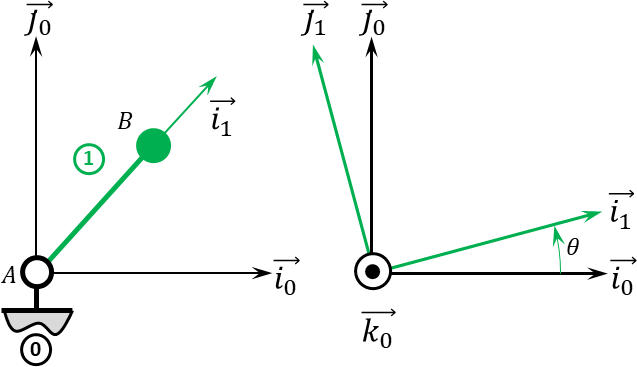
\includegraphics[width=\linewidth]{02_R_01}
\end{marginfigure}
\fi

\question{Réaliser le paramétrage du mécanisme.}
\ifprof ~\\

\else
\fi


\ifprof
\else
\marginnote{Corrigé voir \ref{CIN:01:B2:13:PTSI:02}.}
\fi